
\documentclass{article}
\usepackage[utf8]{inputenc}
\usepackage{graphicx}
\usepackage[T1]{fontenc}
\usepackage{lmodern}
\usepackage{listings}
\usepackage[numbers]{natbib} %IEEE
\usepackage{color}
\usepackage{hyperref}
\usepackage{soul}
\usepackage{float}
\usepackage{pgfplotstable}
\usepackage[font=itshape]{quoting}
\usepackage{booktabs}
\usepackage{amsmath}
\setcounter{MaxMatrixCols}{13}
\usepackage{multicol}
%\usepackage[table,xcdraw]{xcolor}

\usepackage{minted}
\usepackage[a4paper, total={6in, 8in}]{geometry}
\definecolor{dkgreen}{rgb}{0,0.6,0}
\definecolor{gray}{rgb}{0.5,0.5,0.5}
\definecolor{mauve}{rgb}{0.58,0,0.82}
\definecolor{backcolour}{rgb}{0.95,0.95,0.92}
\definecolor{codegreen}{rgb}{0,0.6,0}
% Define a custom style
\lstdefinestyle{myStyle}{
    backgroundcolor=\color{backcolour},   
    commentstyle=\color{codegreen},
    keywordstyle = \bfseries\color{mauve},
    basicstyle=\ttfamily\footnotesize,
    breakatwhitespace=false,         
    breaklines=true,                 
    keepspaces=true,                 
    numbers=left,       
    numbersep=5pt,                  
    showspaces=false,                
    showstringspaces=false,
    showtabs=false,                  
    tabsize=2,
}
\lstset{style=mystyle}

\title{Data Mining \& Machine Learning \\ \large Computer Exercise 8 - Support Vector Machines}
\author{Steinarr Hrafn Höskuldsson}
\date{October 2022}
\newcommand{\mycomment}[1]{}

\begin{document}
\maketitle
\mycomment{
\begin{figure}[H]
    \centering
    \includegraphics[width=0.75\textwidth]{LAB3/Basic1.png}
    \caption{"Switch test" Breadboard set up}
    \label{fig:Switch_test}
\end{figure}

\lstinputlisting[caption=Defining 'ColorMatch' state, label={lst:colormatch}, language=Python, firstline=44, lastline=52]{LAB3/Basic.py}

}


\section*{Section 1.2}

The confusion matrix was :

\\
\begin{center}
CM = \begin{bmatrix}
    61 & 2 \\
    4 & 104 \\
\end{bmatrix}\\
\end{center}
\\

Accuracy was 96.5\%, Precision was 98.1\%, recall was 96.3\% and cross validation accuracy was 91.5\%. 

Precision and recall gives a better picture than accuracy regarding false positives and false negatives. For an issue such as detecting cancer a false positive is preferable over a false negative. In such a case we want a model with high recall. 

There is a noticeable discrepancy between accuracy and cross validation accuracy. By random chance the test/train split of the data set happened to result in a favourable set for the model, it's unlikely the model will get lucky 10 times in a row thus the cross validation score gives a much more accurate view of the accuracy.

If we wanted a confusion matrix from the cross validation we could implement our own cross validation method that averages up the confusion matrices into one. Precision and recall could then be calculated from the averaged confusion matrix.

\section*{Section 2.1}
The confusion matrix was:

          \begin{center}
          CM= \begin{bmatrix}
          59 & 4 \\
          0  & 108 
          \end{bmatrix}
          \end{center}


          Accuracy was 97.66\% , Precision was 96.43\% , recall was 100.00\% and cross validation accuracy was 96.14\% .
          
The best combination of hyperparameters found were \verb!n_estimators = 120! and \verb!max_features = 4!.

\section*{Section 2.2}
\begin{figure}[H]
    \centering
    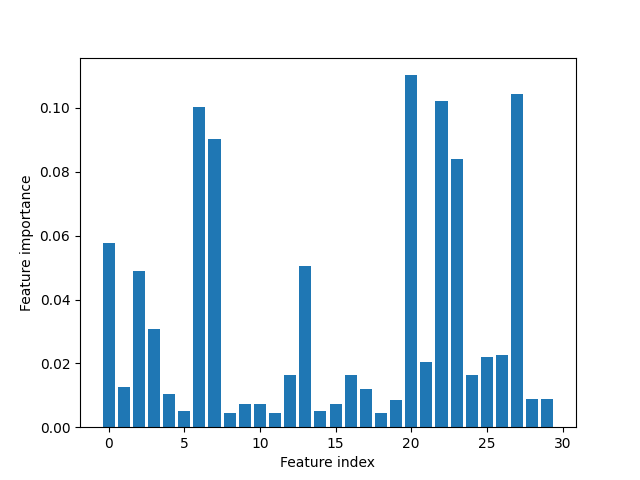
\includegraphics[width=0.75\textwidth]{09_random_forests/2_2_1.png}
    \caption{}
    \label{fig:Switch_test}
\end{figure}

\section*{Section 2.3}
The most important feature was the 23rd feature, number 22, named \verb!compactness_worst!. The least important feature was the ninth feature, number 8, named \verb!symmetry_mean!

\section*{Section 2.4}
\begin{figure}[H]
    \centering
    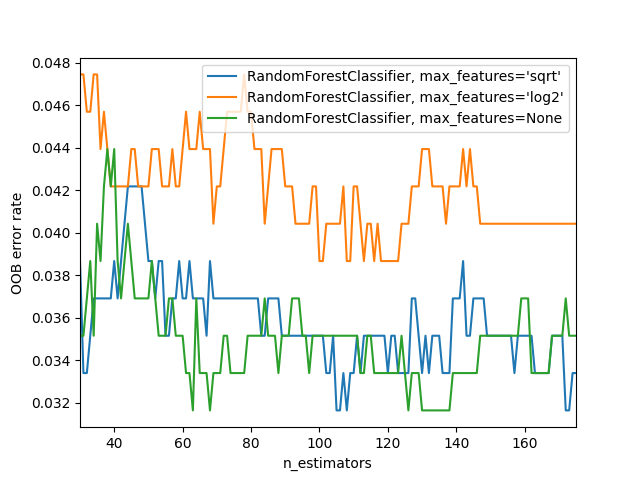
\includegraphics[width=0.75\textwidth]{09_random_forests/2_4_1.png}
    \caption{The Out Of Bag error for different settings of parameters. The plots have been smoothed slightly using scipy's uniformfilter1d function, using n=5.}
    \label{fig:24}
\end{figure}

\section*{Section 2.5}
Looking at Figure \ref{fig:24} there does not seem to be a correlation between \verb"n_estimators" and the Error rate.

This seems to be true for all three types of ensambles.

\section{Section 3.1}
\begin{figure}[H]
    \centering
    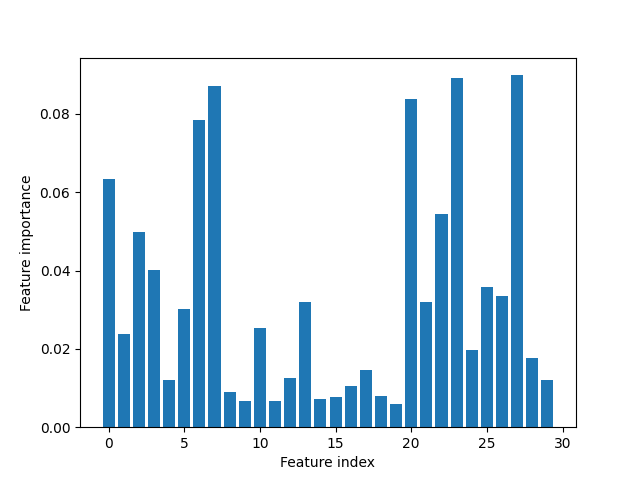
\includegraphics[width=0.75\textwidth]{09_random_forests/3_1_1.png}
    \caption{the Feature importance for Extremely Random Forest}
    \label{fig:31}
\end{figure}
The confusion matrix was:

          \begin{center}
          CM= \begin{bmatrix}
          58 & 5 
          0  & 108 
          \end{bmatrix}
          \end{center}


          Accuracy was 97.08\% , Precision was 95.58\% , recall was 100.00\% and cross validation accuracy was 97.01\% 



\section{Section 3.2}
\begin{figure}[H]
    \centering
    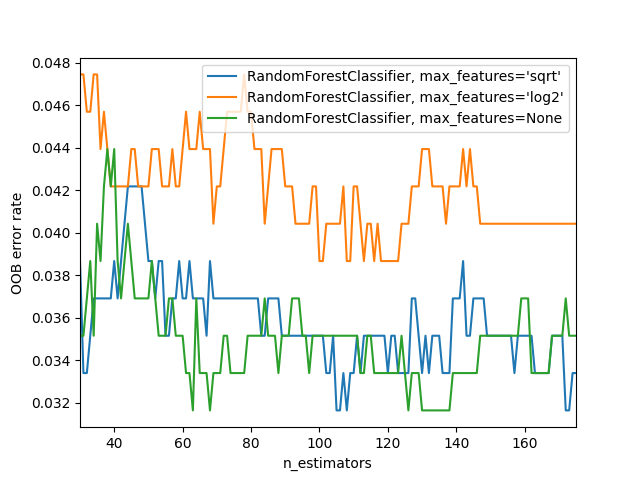
\includegraphics[width=0.75\textwidth]{09_random_forests/2_4_1.png}
    \caption{The Out Of Bag error for different settings of parameters of Extremely Random Forest Classifier. The plots have been smoothed slightly using scipy's uniformfilter1d function, using n=5.}
    \label{fig:32}
\end{figure}

\section*{Independent}

\newpage
\section*{Appendix}
\appendix
\section{Code}

\lstinputlisting[caption={The code used}, language=Python, ]{08_SVM/Steinarr8.py}



\end{document}

